\documentclass[a4paper, 12pt]{article}

\usepackage[table,xcdraw]{xcolor}
\usepackage{enumerate}
\usepackage{graphicx}
\usepackage[T5]{fontenc}
\usepackage[utf8]{inputenc}
\usepackage[margin = 2cm]{geometry}
\usepackage{amsfonts, amsmath, amssymb}
\usepackage[none]{hyphenat}
\usepackage{fancyhdr}
\usepackage{float}
\usepackage{hyperref}
\usepackage{physics}
\usepackage{caption}
\usepackage{subcaption}
\usepackage[nottoc, notlot, notlof]{tocbibind}

\usepackage{mathtools}
\DeclarePairedDelimiter\ceil{\lceil}{\rceil}
\DeclarePairedDelimiter\floor{\lfloor}{\rfloor}
% for code section
\usepackage{listings}

% for sub-figure
\usepackage{subcaption}
% \usepackage{rotating}
% \usepackage{tikz}

\captionsetup[table]{skip=5pt}
\pagestyle{fancy}
\fancyhead[L]{Trường Đại học Khoa học Tự nhiên - ĐHQG TP.HCM}
\fancyhead[R]{Nhóm 9}

% Paragraph format
\setlength{\parindent}{0em}
\setlength{\parskip}{1em}

\begin{document}

\begin{titlepage}
    \begin{center}
        %\vspace*{1cm}
        \Large\textbf{Đại học Quốc gia TP. HCM\\Trường Đại học Khoa học Tự nhiên\\Bộ Môn Khoa học Máy tính}\\

        \vspace*{1cm}
        \begin{figure}[H]
            \begin{center}
                
\includegraphics[scale=0.2]{img/hcmus-logo}
            \end{center}
        \end{figure}
        \line(1,0){450}\\[4mm]
        \LARGE\textbf{\MakeUppercase{Báo cáo Seminar Cuối kì\\ Face Recognition}}\\[3mm]
        \Large{Nhận Dạng (CSC14006)}\\[3mm]
        \Large{Nhóm 9}
        \line(1,0){430}\\

        \vfill
        TP Hồ Chí Minh, ngày 01/06/2021
    \end{center}
\end{titlepage}

\tableofcontents
\thispagestyle{empty}
\clearpage

\section{Thông tin nhóm}
    \begin{table}[H]
        \centering
        \begin{tabular}{|c|c|l|c|c|}
        \hline
        STT & MSSV     & \multicolumn{1}{c|}{Họ tên} & Email\\ \hline
        1   & 18120078 & Ngô Phù Hữu Đại Sơn         & 18120078@student.hcmus.edu.vn\\ \hline
        2   & 18120533 & Dương Đoàn Bảo Sơn          & 18120533@student.hcmus.edu.vn\\ \hline
        3   & 18120164 & Lê Minh Đức                 & 18120164@student.hcmus.edu.vn\\ \hline
        \end{tabular}
        \caption{Bảng danh sách thành viên nhóm}
    \end{table}

\section{Phân công các thành viên trong nhóm}

    \begin{table}[H]
        \centering
        \begin{tabular}{|c|l|l|c|}
        \hline
        STT & \multicolumn{1}{c|}{Họ tên} & \multicolumn{1}{c|}{Công việc tham gia}  & Hoàn thành (\%) \\ \hline
        1   & Ngô Phù Hữu Đại Sơn         & CNNS, ResNet và ArcFace loss             & 100/100 \\ \hline
        2   & Dương Đoàn Bảo Sơn          & Databases                                & 100/100 \\ \hline
        5   & Lê Minh Đức                 & Các kỹ thuật cơ bản nhận dạng            & 100/100 \\ \hline
        \end{tabular}
        \caption{Bảng phân tích tỷ lệ hoàn thành công việc}
    \end{table}
    \clearpage

\section{Mở Đầu}
Các hệ thống nhận dạng khuôn mặt ngày nay vai trò quan trọng trong nhiều lĩnh vực ví dụ như giúp nhận dạng các phần tử khủng bố. Ngoài ra chúng còn giúp tăng tính bảo mật của các hệ thống bảo mật ngày nay. Tuy nhiên để có thể xây dựng đươc một hệ thống nhạn diện khuôn mặt hiệu quả vẫn còn là một thách thức trong lĩnh vực nghiên cứu. Những vấn đề mà ta đang gặp phải như sự thay đổi của gương mặt thông qua biểu cảm, tư thế gương mặt, lão hóa, trang điểm, sử dụng mắt kính, khẩu trang,... Ngoài ra các điều kiện chiếu sáng và góc chụp khác nhau cũng dẫn đến các lỗi trong nhận diện. Trong  báo cáo này, nhóm em xin trình bày các kĩ thuật cơ bản và cổ điển trong các bài toán nhận diện khuôn mặt như \textit{Pricipal Component Analysis (PCA), Linear Disciminant Analysis (LDA)} và \textit{Support Vector Machine (SVM)}. Sau đó, nhóm sẽ trình bày các tập dữ liệu kinh điển (\textit{FGRC, FERET,...}) và một số tập dữ liệu mới ngày nay (\textit{LFW, CFP-FP, AgeDB,...}). Cuối cùng, nhóm em xin trình bày kĩ thuật mới và hiện đại hơn trong nhận diện gương mặt là \textit{Convolutional Neural Network(CNNs)} - cấu trúc mạng học sâu quen thuộc ngày nay trong các bài toán về thị giác máy tính, \textit{Residual Network (ResNet)} - Cấu trúc giúp tối ưu mạng học sâu có nhiều lớp và \textit{ArcFace Loss} giúp các hệ thống phân lớp gương mặt hiệu quả hơn. Nhóm em còn thực hiện thêm một demo sử dụng \textit{ArcFace} giải quyết bài toán \textit{Face Verification} để có cái nhìn rõ hơn về phương pháp đã nêu trên.

\begin{figure}[ht]
    \subfloat[Face Generation]{
      \begin{minipage}[c][1\width]{ 0.3\textwidth}
         \centering
         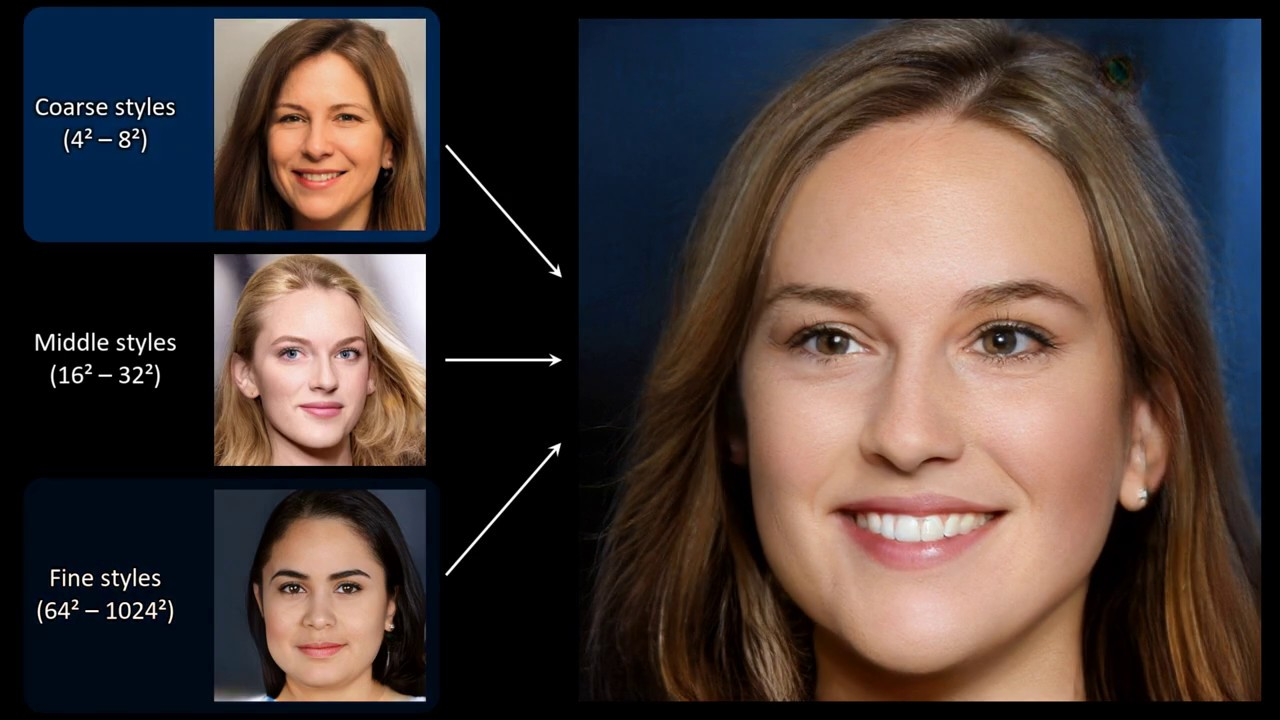
\includegraphics[width=1\textwidth]{img/face-generation}
      \end{minipage}}
   \hfill 	
    \subfloat[Face Identification]{
      \begin{minipage}[c][1\width]{ 0.3\textwidth}
         \centering
         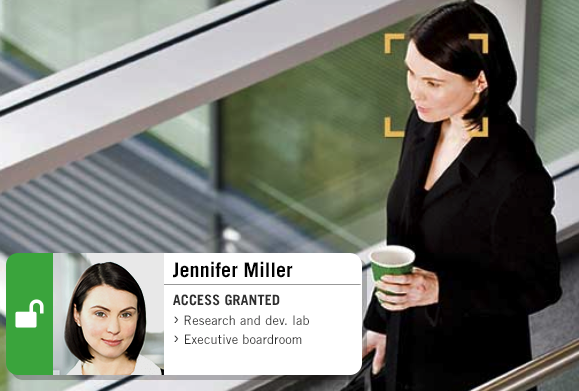
\includegraphics[width=1.0\textwidth]{img/face-identification}
      \end{minipage}}
   \hfill	
    \subfloat[Face Verification]{
      \begin{minipage}[c][1\width]{ 0.3\textwidth}
         \centering
         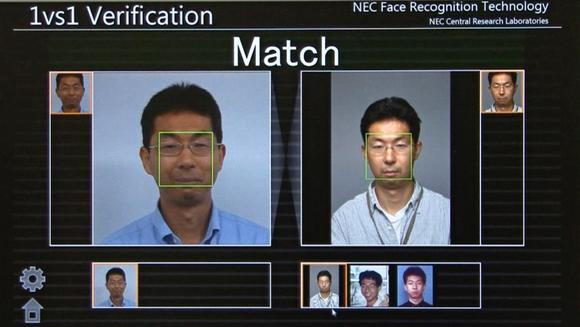
\includegraphics[scale=0.5, width=1\textwidth]{img/face-verification}
      \end{minipage}}
  \caption{Một số ứng dụng của nhận diện gương mặt}
  \end{figure}
\clearpage

\section{Các Kĩ Thuật Cơ Bản}
\subsection{Phân tích thành phần chính (Principal Component Analysis - PCA)}
\subsubsection{Tổng quan về PCA}

PCA là kĩ thuật giảm chiều dữ liệu từ n chiều sang dữ liệu m chiều (m<n) mà vẫn giữ được nhiều thông tin nhất có thể.
\begin{figure}[H]
    \begin{center}
        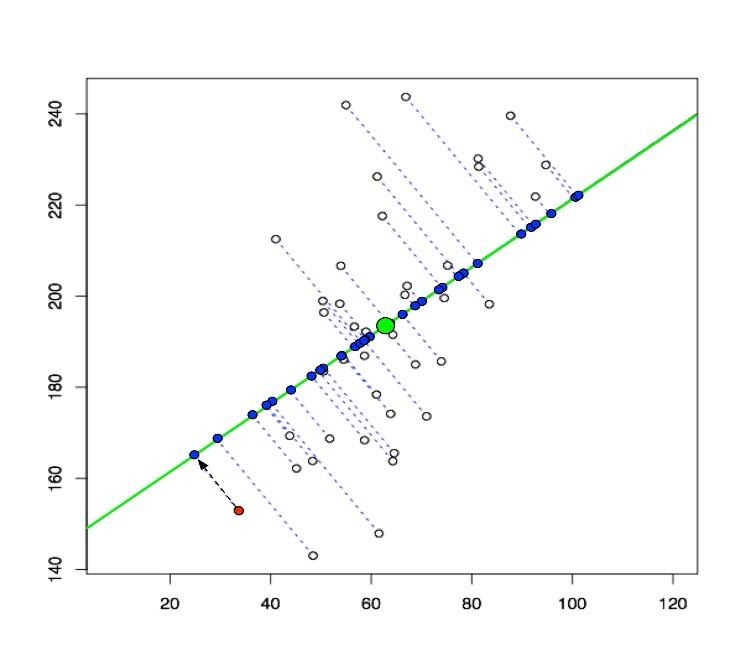
\includegraphics[scale=0.5]{img/PCA-example}
        \caption{Minh họa PCA}
    \end{center}
\end{figure}

\subsubsection{Cách bước tính của PCA}
\begin{itemize}
    \item Bước 1: Tính giá trị trung bình: $\bar{x}=\frac{1}{N}\sum_{n=1}^{N}{x_n}$.
    \item Bước 2: Chuẩn hóa: $\hat{x} = x_n - \bar{x}$.
    \item Bước 3: Tính ma trận hiệp phương sai: $S = \frac{1}{N}\hat{X}\hat{X}^T$.
    \item Bước 4: Tính các trị riêng $\lambda_i$ và vector riêng $v_i: Sv_i=\lambda_iv_i$.
    \item Bước 5: Chọn K vector riêng ứng với K trị riêng lớn nhất để xây dựng ma trận $U_K$ có các cột tạo thành một hệ trực giao. K vector này, còn được gọi là các thành phần chính, tạo thành một không gian con gần với phân bố của dữ liệu ban đầu đã chuẩn hoá.
    \item Bước 6: Chiếu dữ liệu ban đầu đã chuẩn hoá X xuống không gian con tìm được. Dữ liệu mới chính là toạ độ của các điểm dữ liệu trên không gian mới: $Z=U_K^T \hat{X}$
\end{itemize}

\subsubsection{Ví dụ minh họa}
Có các điểm sau (2.5, 2.4), (0.5, 0.7), (2.2, 2.9), (1.9, 2.2), (3.1,3.0), (2.3, 2.7), (2, 1.6), (1, 1.1), (1.5, 1.6), (1.1, 0.9). Sử dụng PCA để giảm chúng về 1 chiều.
\begin{itemize}
    \item Bước 1: Tính trung bình, chuẩn hóa.
    \begin{figure}[H]
        \begin{center}
            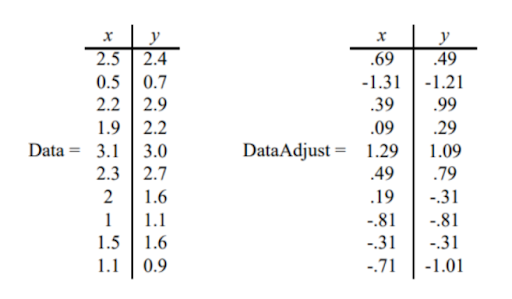
\includegraphics[scale=0.5]{img/PCA-cal-1}
            \caption{Tính trung bình, chuẩn hóa}
        \end{center}
    \end{figure}

    \item Bước 2: Ma trận hiệp phương sai.
    \begin{figure}[H]
        \begin{center}
            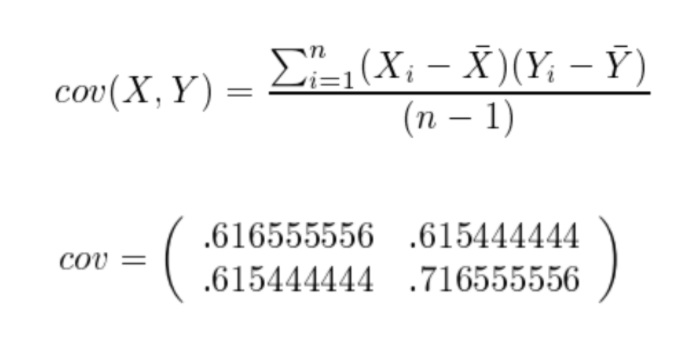
\includegraphics[scale=0.5]{img/PCA-cal-2}
            \caption{Ma trận hiệp phương sai}
        \end{center}
    \end{figure}
    
    \item Bước 3: Tính vector riêng và giá trị riêng cho ma trận hiệp phương sai.
    \begin{figure}[H]
        \begin{center}
            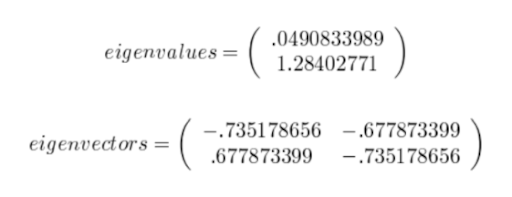
\includegraphics[scale=0.5]{img/PCA-cal-3}
            \caption{Ma trận hiệp phương sai}
        \end{center}
    \end{figure}
    
    \item Bước 4: Biến đổi dữ liệu:
    \begin{figure}[H]
        \begin{center}
            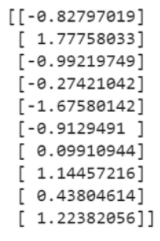
\includegraphics[scale=0.5]{img/PCA-cal-4}
            \caption{Dữ liệu sao khi biến đổi}
        \end{center}
    \end{figure}
\end{itemize}

\begin{figure}[H]
    \begin{center}
        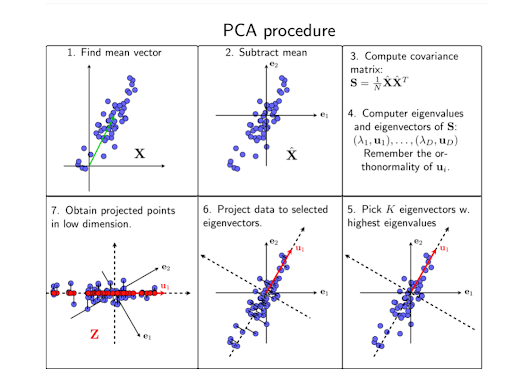
\includegraphics[scale=0.7]{img/PCA-total}
        \caption{Tổng kết toàn bộ quá trình PCA}
    \end{center}
\end{figure}

\subsection{Phân tích biệt thức tuyến tính (Linear Discriminant Analysis - LDA)}
\subsubsection{Tổng quan về LDA}

LDA là một thuật toán học có giám sát, giảm chiều dữ liệu.

Mục đích LDA là tìm sự khác nhau giữa các thành phần trong 1 class (within-class) là nhỏ và sự khác nhau giữa các classes là lớn.

Khác với PCA, LDA tìm phép chiếu sao cho tối đa hóa sự khác biệt giữa các lớp để có thể phân lớp hiệu quả.

\begin{figure}[H]
    \begin{center}
        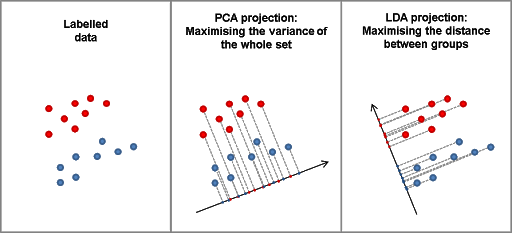
\includegraphics[scale=0.7]{img/LDA-PCA-cmp}
        \caption{So sánh LDA và PCA (1)}
    \end{center}
\end{figure}

\subsubsection{Các bước tính của LDA}

\begin{itemize}
    \item Bước 1: Tính ma trận phân tán giữa các nhóm.
    \begin{equation}
        S_B=\sum_{i=1}^{C}{n_i(\mu_i - \mu)(\mu_i-\mu)^T}
    \end{equation}
    \subitem $\mu_i$ là giá trị trung bình của từng lớp. 
    \subitem $\mu$ là giá trị trung bình của tất cả dữ liệu. 

    \item Bước 2: Tính ma trận phân tán tích lũy ứng với từng nhóm.
    \begin{equation}
        S_W=\sum_{j=1}^{C}{\sum_{i=1}^{n_j}{(x_{ij}-\mu_j)(x_{ij}-\mu_j)^T}}
    \end{equation}

    \item Bước 3: Xây dựng hàm tiêu chí tách lớp.
    \begin{equation}
        W = S_W^{-1}S_B
    \end{equation}

    \item Bước 4: Dự đoán nhãn của mẫu dữ liệu nhập (so sánh vector trung bình của từng nhóm – gần vector trung bình nhất).
\end{itemize}

\subsubsection{Ví dụ minh họa}

\begin{figure}[H]
    \begin{center}
        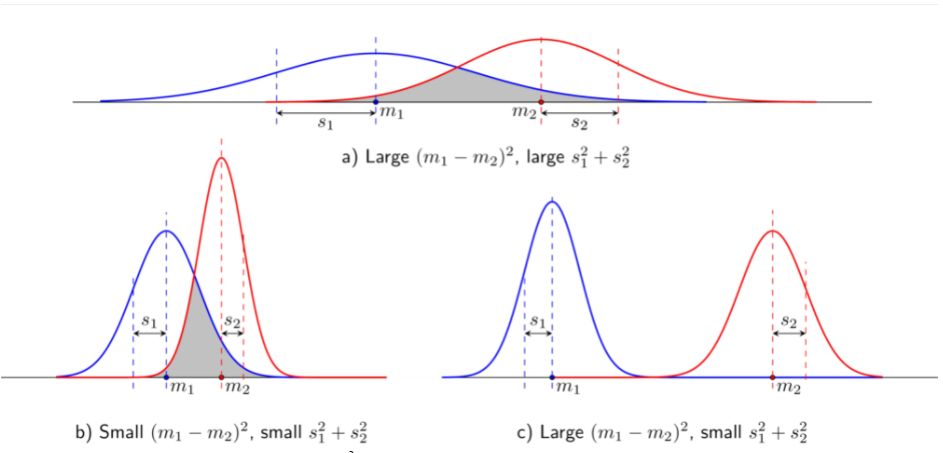
\includegraphics[scale=0.3]{img/LDA-example-1}
        \caption{Ví dụ minh họa LDA}
    \end{center}
\end{figure}

Hình trên là khoảng cách giữa các kỳ vọng và tổng các phương sai ảnh hưởng tới độ phân biệt của dữ liệu. a) Khoảng cách giữa hai kỳ vọng là lớn nhưng phương sai trong mỗi class cũng lớn, khiến cho hai phân phối chồng lấn lên nhau (phần màu xám). b) Phương sai cho mỗi class là rất nhỏ nhưng hai kỳ vọng quá gần nhau, khiến khó phân biệt 2 class. c) Khi phương sai đủ nhỏ và khoảng cách giữa hai kỳ vọng đủ lớn, ta thấy rằng dữ liệu phân biệt hơn.


\begin{figure}[ht]
    \subfloat[Tối ưu khoảng cách trong LDA]{
      \begin{minipage}[c][1\width]{ 0.3\textwidth}
         \centering
         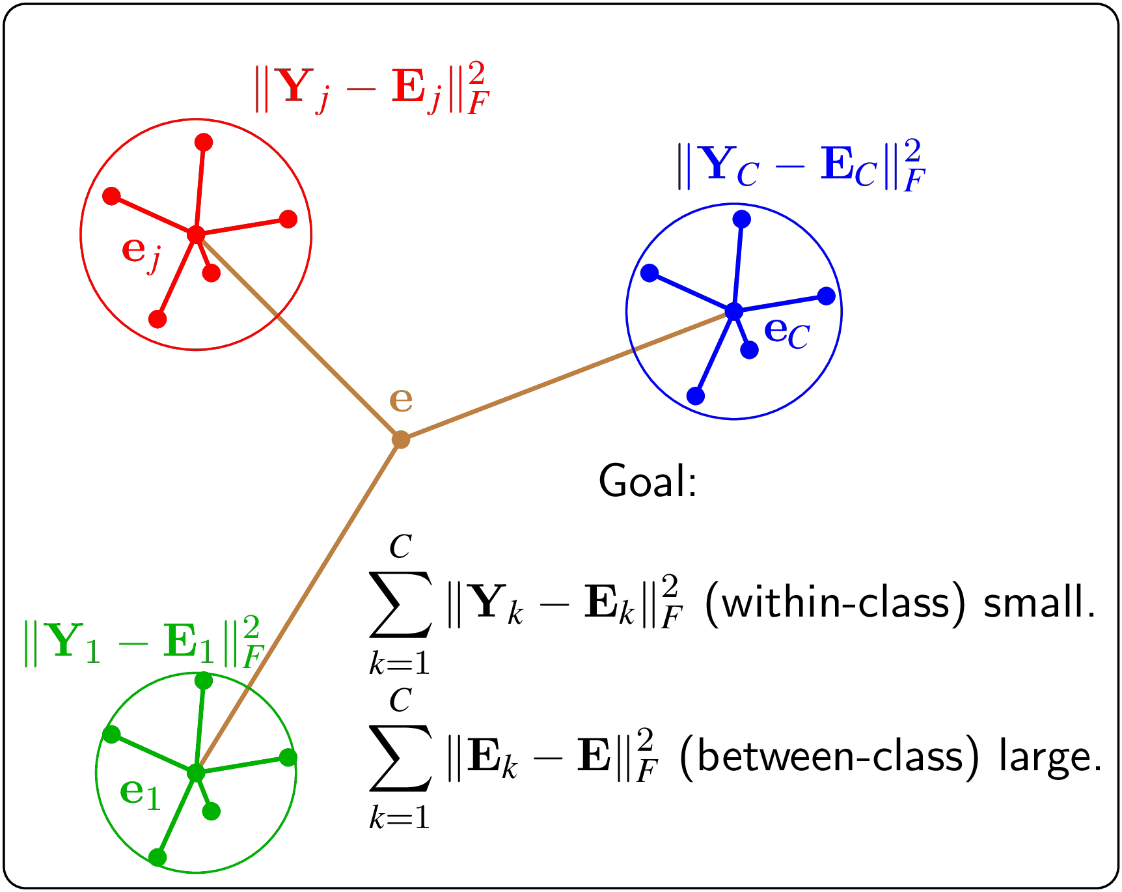
\includegraphics[width=1\textwidth]{img/LDA-example-2}
      \end{minipage}}
   \hfill 	
    \subfloat[So sánh PCA và LDA (2)]{
      \begin{minipage}[c][1\width]{ 0.3\textwidth}
         \centering
         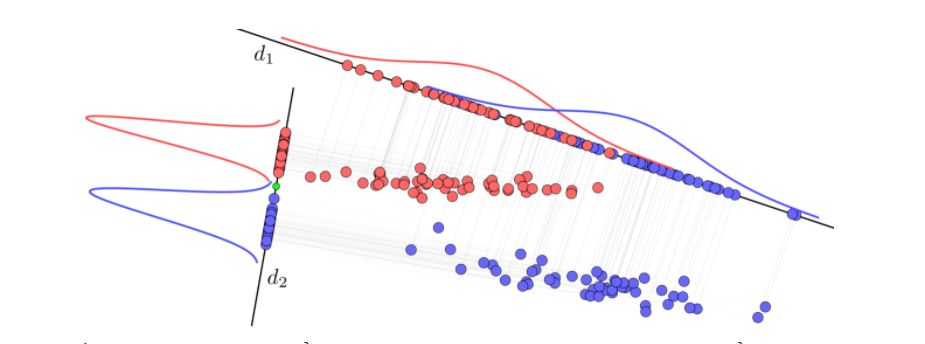
\includegraphics[width=1.0\textwidth]{img/LDA-example-3}
      \end{minipage}}
   \hfill	
    \subfloat[So sánh PCA và LDA (3)]{
      \begin{minipage}[c][1\width]{ 0.3\textwidth}
         \centering
         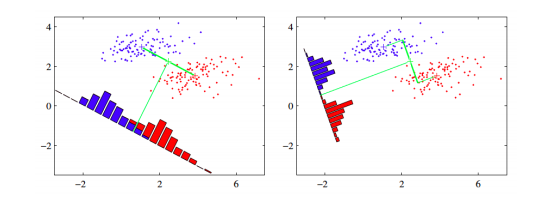
\includegraphics[scale=0.5, width=1\textwidth]{img/LDA-example-4}
      \end{minipage}}
  \caption{Một số hình ảnh ví dụ về LDA}
  \end{figure}
\clearpage

\subsection{Support Vector Machine – SVM}
\subsubsection{Tổng quan về SVM}
SVM là một thuật toán giám sát, nó có thể sử dụng cho cả việc phân loại hoặc hồi quy.

SVM là tìm một siêu phẳng (hyperplane) để phân tách các điểm dữ liệu thành 2 lớp riêng biệt, ta cần phải tối ưu hóa siêu phẳng này.

SVM dùng thủ thuật để ánh xạ bộ dữ liệu đó vào không gian nhiều chiều hơn (n chiều), từ đó tìm ra siêu phẳng (hyperplane) để phân chia.

Đối với dữ liệu 2 chiều, hyperplane là 1 đường thẳng; dữ liệu 3 chiều là 1 mặt phẳng, \dots

\begin{figure}[H]
    \begin{center}
        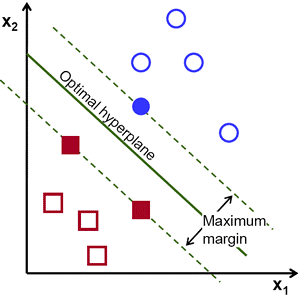
\includegraphics[scale=0.3]{img/SVM-ex-1.png}
        \caption{Minh họa SVM}
    \end{center}
\end{figure}

\subsubsection{Các bước tính của SVM}
\begin{itemize}
    \item Chọn hàm \textit{Kernel}.
	\item Chọn giá trị điều khiển biến cho dữ liệu huấn luyện C.
	\item Bài toán tối ưu bậc hai để tìm tham số cho vector hỗ trợ.
	\item Xây dựng hàm tách lớp từ các vector hỗ trợ.
\end{itemize}

\subsubsection{Ví dụ minh họa SVM}
\begin{itemize}
    \item Đối với dữ liệu tuyến tính:
    \begin{figure}[H]
        \begin{center}
            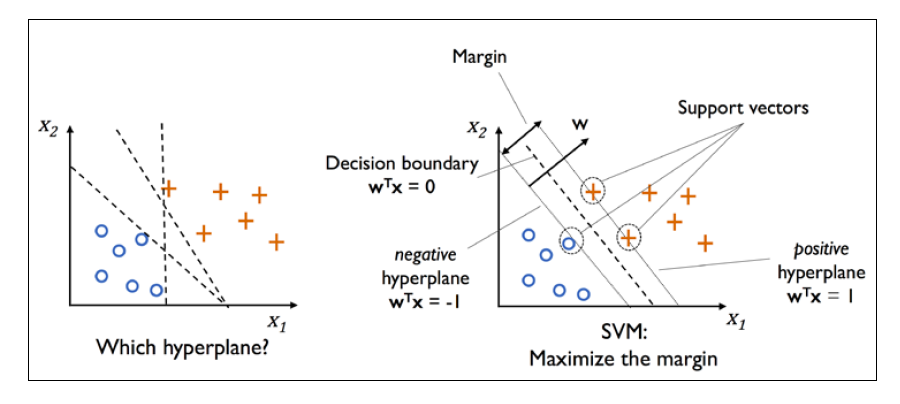
\includegraphics[scale=0.3]{img/SVM-ex-2}
            \caption{SVM với dữ liệu tuyến tính}
        \end{center}
    \end{figure}

    \item Đối với dữ liệu phi tuyến ta không thể chia trực tiếp bằng các đường thẳng, ta cần phải sử dụng hàm \textit{Kernel} để ánh xạ dữ liệu đó vào không gian nhiều chiều hơn:
    \begin{figure}[H]
        \begin{center}
            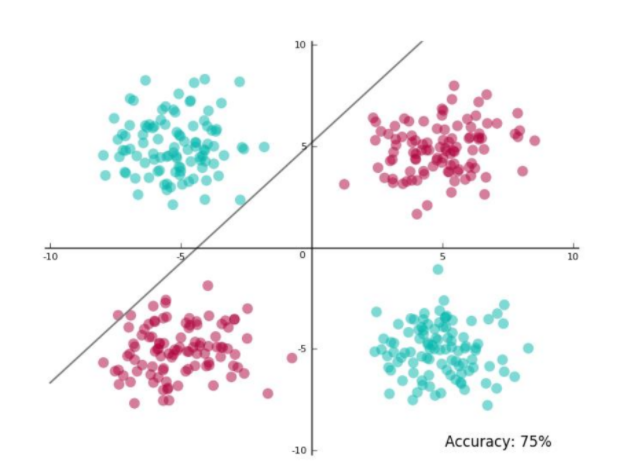
\includegraphics[scale=0.3]{img/SVM-kernel-1}
            \caption{SVM với dữ liệu phi tuyến}
        \end{center}
    \end{figure}
    \subitem Ta sử dụng hàm \textit{Kernel} để ánh xạ tập dữ liệu 2 chiều trên thành dữ liệu 3 chiều từ đó dễ dàng tìm ra siêu phẳng để phân lớp hơn.
    \begin{figure}[H]
        \begin{center}
            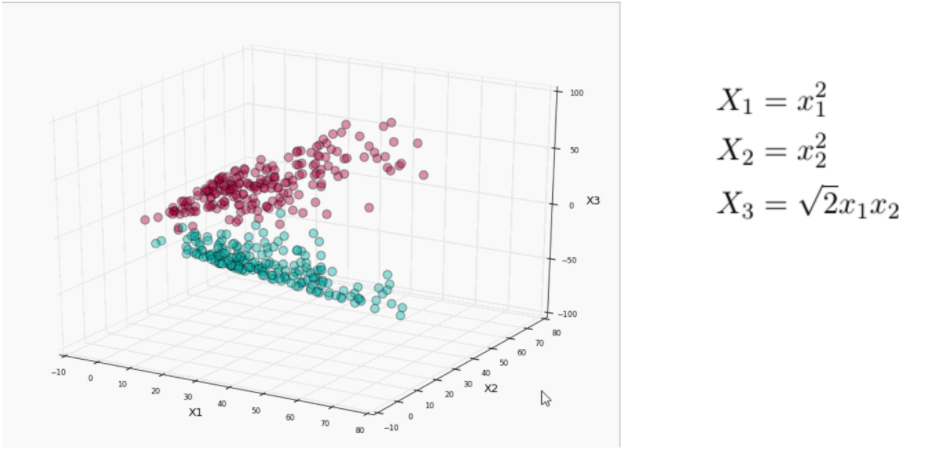
\includegraphics[scale=0.3]{img/SVM-kernel-2}
            \caption{Tăng chiều dữ liệu bằng các hàm kernel}
        \end{center}
    \end{figure}
\end{itemize}

\subsubsection{Một số hàm kernel thông dụng}
\begin{itemize}
    \item Hàm tuyến tính: $K(x_i, x_j) = x_i^Tx_j$.
    \item Hàm đa thức: $K(x_i, x\_j) = (1 + x_i^Tx_j)^p$
    \item Gaussian: $K(x_i, x_j) = e^{-\frac{\|x_i-x_j\|^2}{2\sigma^2}}$.
    \item Sigmoid: $K(x_i, x_j) = tanh(\beta_0x_i^Tx_j + \beta_1)$
\end{itemize}

\section{Các cơ sở dữ liệu}
\subsection{FRGC database}

Dữ liệu cho Face Recognition Grand Challenge database (FRGC) là bộ dataset lớn bao gồm 50.000 bản ghi được chia thành tập training và validation.\par
Tập validation bao gồm dữ liệu từ 4.003 subject sessions. Một subject sessions là tập hợp tất cả các hình ảnh của một người được chụp qua mỗi lần thu thập dữ liệu sinh trắc học và gồm có 4 hình ảnh tĩnh được kiểm soát, 2 hình ảnh tĩnh không được kiểm soát và 1 hình ảnh ba chiều.

Các hình ảnh được kiểm soát được chụp trong bối cảnh studio, là hình ảnh toàn bộ khuôn mặt trực diện được chụp trong hai điều kiện ánh sáng và với hai biểu cảm khuôn mặt (tươi cười và trung tính).

Các hình ảnh không được kiểm soát được chụp trong các điều kiện ánh sáng khác nhau; ví dụ: hành lang, nhĩ thất hoặc bên ngoài. Mỗi bộ ảnh không kiểm soát có hai biểu cảm(tươi cười và trung tính).

Hình ảnh 3D được chụp trong điều kiện ánh sáng được kiểm soát. Hình ảnh 3D được thu thập bởi  Minolta Vivid 900/910 series sensor.

    \begin{figure}[H]
        \begin{center}
            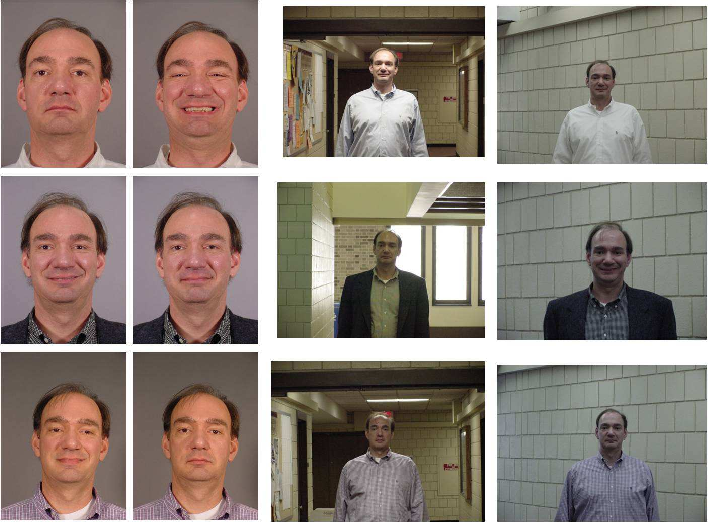
\includegraphics[scale=0.5]{img/FRGC.png}
            \caption{Ảnh chụp có kiểm soát (trái) và ảnh chụp không kiểm soát (phải)}
        \end{center}
    \end{figure}

\subsection{FERET database}
The Facial Recognition Technology (FERET) database được sử dụng để đánh giá hệ thống nhận dạng khuôn mặt là một phần của the Face Recognition Technology program.

FERET database được thu thập trong  từ tháng 12 năm 1993 đến tháng 8 năm 1996. 

Cơ sở dữ liệu chứa 1564 bộ ảnh trong tổng số 14,126 ảnh bao gồm 1199 người và 365 bộ ảnh trùng lặp.

Bộ ảnh trùng lặp là tập hợp hình ảnh thứ hai của một người đã có trong cơ sở dữ liệu và thường được chụp vào một ngày khác.

    \begin{figure}[H]
        \begin{center}
            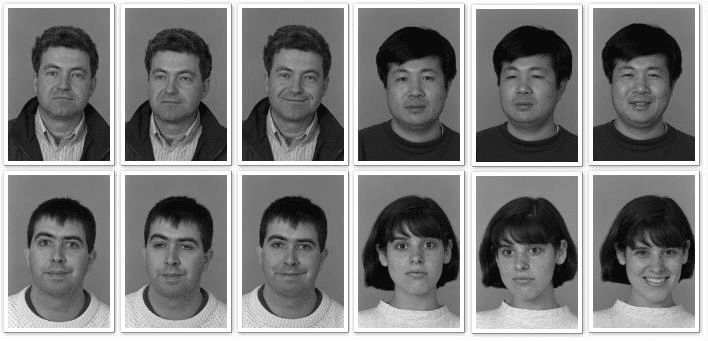
\includegraphics[scale=0.5]{img/FERET.png}
            \caption{Ảnh của các đối tượng được chụp trong ngày khác nhau}
        \end{center}
    \end{figure}

\subsection{PIE database}
CMU Pose, Illumination and Expression (PIE) database được thu thập giữa tháng 10 và 12/2000

PIE database chứa 41.368 hình ảnh khuôn mặt của 68 người.

Các hình ảnh có được trên các tư thế, dưới các ánh sáng và với các nét mặt khác nhau. 

Hình ảnh của mỗi người được chụp dưới 13 tư thế khác nhau, 43 điều kiện chiếu sáng khác nhau và 4 loại nét mặt.

    \begin{figure}[H]
        \begin{center}
            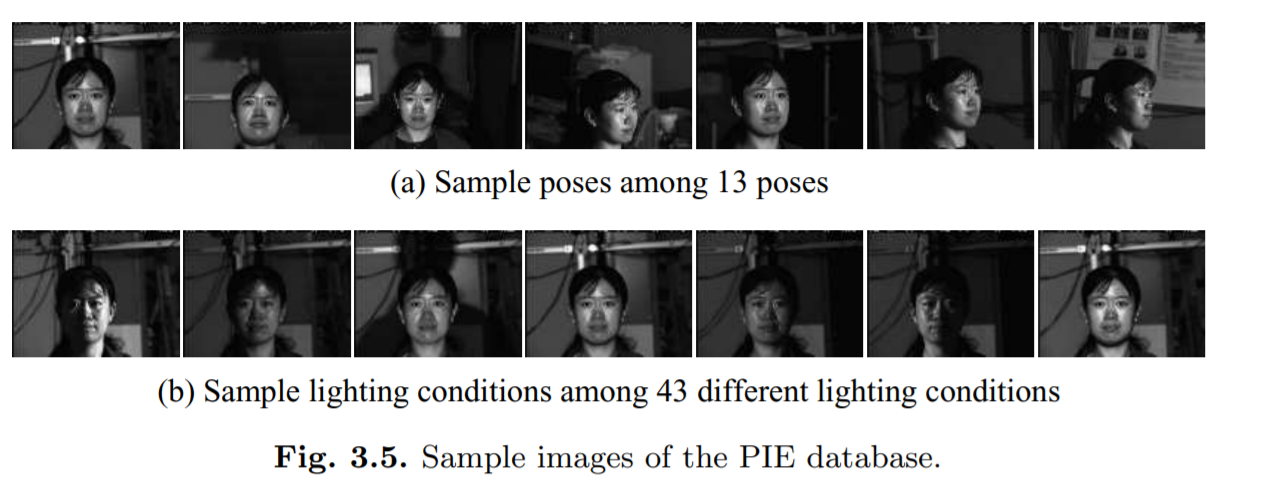
\includegraphics[scale=0.35]{img/PIE.png}
            \caption{Ảnh trong PIE}
        \end{center}
    \end{figure}

\subsection{AR database}
AR database được tạo ra bởi Aleix Martinez and Robert Benavente tại the Computer Vision Center (CVC) của the U.A.B.

Gồm hơn 4000 ảnh màu tương ứng với khuôn mặt của 126 người(70 nam và 56 nữ). 

Hình ảnh trực diện khuôn mặt với các biểu cảm, điều kiện ảnh sáng và sự che khuất(kính và khăn quàng cổ) khác nhau.

    \begin{figure}[H]
        \begin{center}
            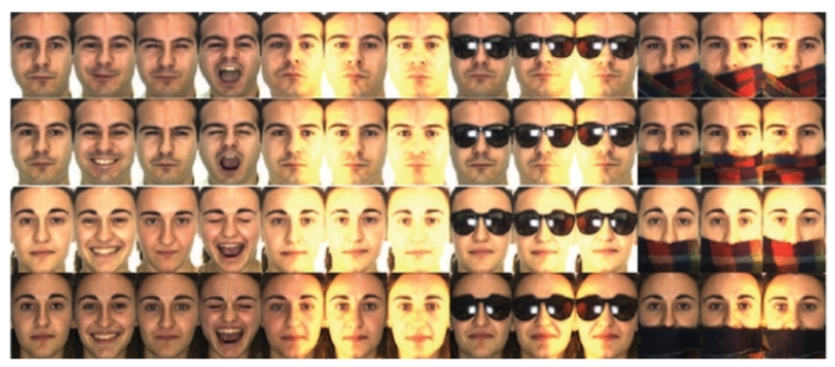
\includegraphics[scale=0.5]{img/AR.png}
            \caption{Ảnh trong AR}
        \end{center}
    \end{figure}

\subsection{Yale Face Database}
Gồm 165 ảnh grayscale ở định dạng GIF của 15 cá nhân.

Có 11 hình ảnh với mỗi cá nhân, cho từng biểu hiện hoặc cấu hình khuôn mặt sau: center-light, w/glasses, happy, left-light, w/no glasses, normal, right-light, sad, sleepy, surprised, and wink.

    \begin{figure}[H]
        \begin{center}
            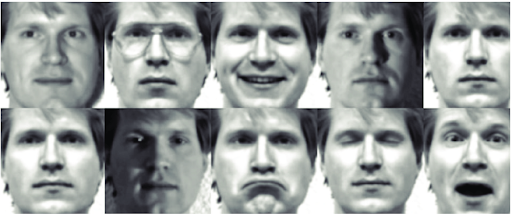
\includegraphics[scale=0.542]{img/Yale1.png}
            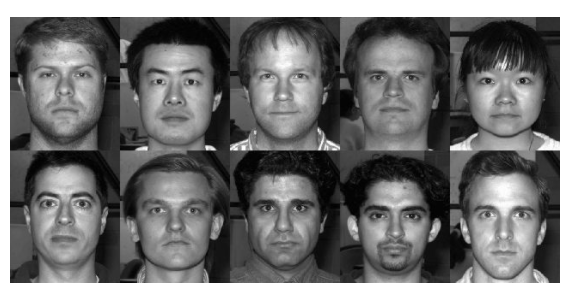
\includegraphics[scale=0.5]{img/Yale2.png}
            \caption{Ảnh trong Yale}
        \end{center}
    \end{figure}
\subsection{MS-CELEB-1M}
Là tập dữ liệu nhận dạng khuôn mặt quy mô lớn bao gồm 100K danh tính và mỗi danh tính có khoảng 100 hình ảnh khuôn mặt. Được lấy từ các công cụ tìm kiếm phổ biến.

Mỗi người được định danh bằng một unique entity key, được liên kết với vài thông tin bao gồm ngày sinh, nghề nghiệp, nơi sinh,…

    \begin{figure}[H]
        \begin{center}
            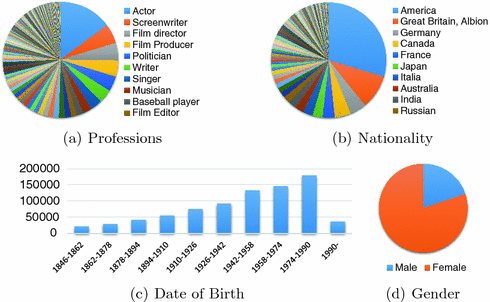
\includegraphics[scale=0.5]{img/MS-CELEB-1M.png}
            \caption{Biểu đồ phân bố dữ liệu trong MS-CELEB-1M}
        \end{center}
    \end{figure}

\subsection{LFW Database}
Bộ dữ liệu bao gồm hơn 13.000 hình ảnh về các khuôn mặt được thu thập từ web của 5749 người có 1 ảnh và 1680 người có 2 ảnh trở lên. Mỗi khuôn mặt đã được dán nhãn với tên của người trong hình.thường được chia thành 2 tập training set và testing set. 

Training set (pairsDevTrain.txt) bao gồm 1100 cặp matched images và 1100 cặp mismatched images.

Testing set (pairsDevTest.txt) bao gồm 500 cặp matched images và 500 cặp mismatched images.

    \begin{figure}[H]
        \begin{center}
            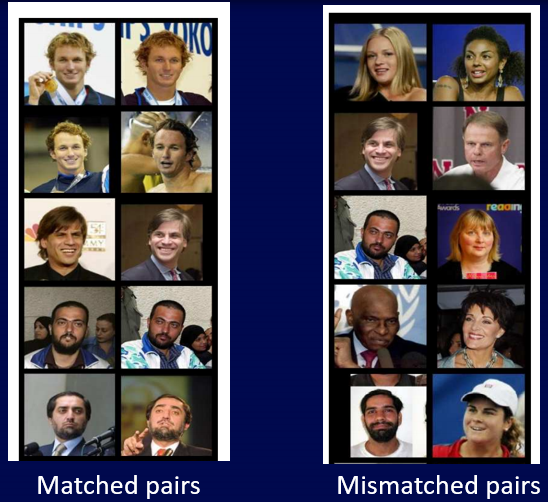
\includegraphics[scale=0.5]{img/LFW.png}
            \caption{Ảnh trong LFW}
        \end{center}
    \end{figure}

\subsection{AgeDB Database}
Dữ liệu được thu thập ở môi trường tự nhiên gồm 16,488 hình ảnh về những người nổi tiếng khác nhau, chẳng hạn như diễn viên, nhà văn, nhà khoa học, chính trị gia, v.v ... Tổng cộng 568 đối tượng.

Số lượng ảnh trung bình cho mỗi đối tượng là 29.

Mọi hình ảnh đều được chú thích liên quan đến danh tính, thuộc tính tuổi và giới tính. 

Độ tuổi tối thiểu và tối đa lần lượt là 1 và 101. Độ tuổi trung bình của mỗi đối tượng là 50,3 tuổi. 

    \begin{figure}[H]
        \begin{center}
            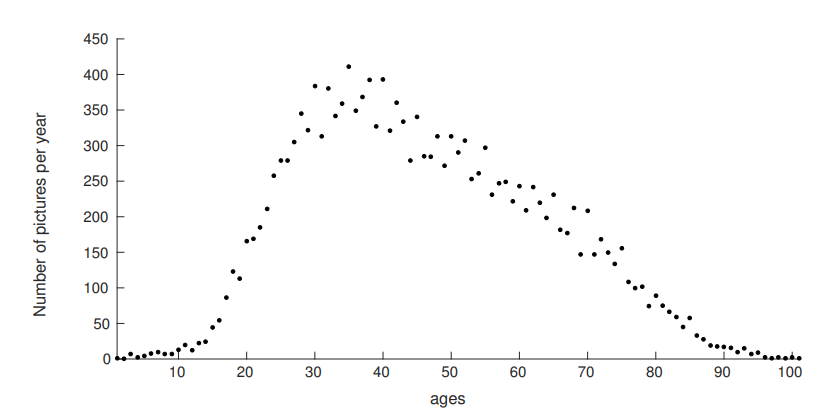
\includegraphics[scale=0.45]{img/AgeDB1}
            \caption{Phân bố  độ tuổi trong AgeDB}
        \end{center}
    \end{figure}

    \begin{figure}[H]
        \begin{center}
            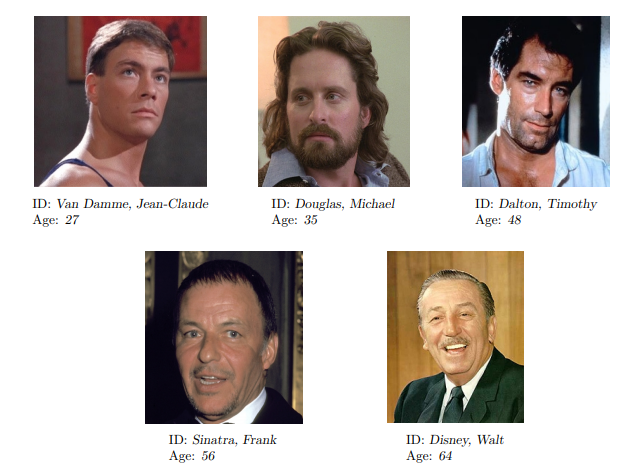
\includegraphics[scale=0.5]{img/AgeDB2}
            \caption{Ảnh trong AgeDB}
        \end{center}
    \end{figure}

\subsection{CFPW Database}
Tập dữ liệu bao gồm 10 ảnh trực diện (Frontal) và 4 ảnh mặt nghiêng (Profile) của 500 cá nhân nổi tiếng. 

Được tách ra 10 phần: mỗi phần gồm 350 cặp giống nhau và 350 cặp khác nhau (tương tự như LFW).

CFP-FP(Frontal-Profile), CFP-FF(Frontal-Frontal) là 2 bộ thử nghiệm được tạo từ CFP database với cách bắt cặp khác nhau (F-P) và (F-F).

    \begin{figure}[H]
        \begin{center}
            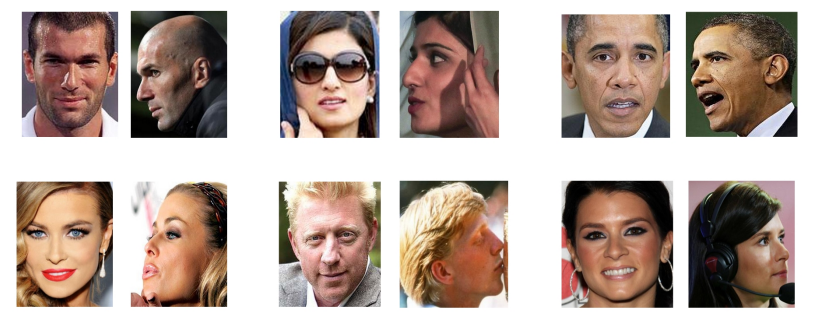
\includegraphics[scale=0.5]{img/CFP.png}
            \caption{Ảnh mẫu một số người nổi tiếng trong CFP}
        \end{center}
    \end{figure}

\section{Mô hình nhận dạng gương mặt ArcFace}
\subsection{Convolutional Neural Network (CNNs)}
\subsubsection{Fully Connected Neural Network}
Fully Connected Neural Network (FCNN) là một mô hình mạng học sâu gồm có nhiều lớp ẩn (hidden layers). Mỗi lớp ẩn sẽ kết nối hoàn toàn (\textit{fully connected}) với lớp trước đó. Kết nối hoàn toàn nghĩa là mọi đầu vào sẽ kết nối với mọi đâu ra. 

Giả sử chúng ta sử dụng FCNN để  để giải quyết bài toán nhận dạng khuôn mặt. Ta cần thực hiện các bước sau: 
\begin{itemize}
    \item Duỗi bức ảnh cần nhận diện thành 1 vector có kích thước (width * height, 1).
    \item Đưa vector đó vào input của FCNN.
\end{itemize}

    \begin{figure}[H]
        \begin{center}
            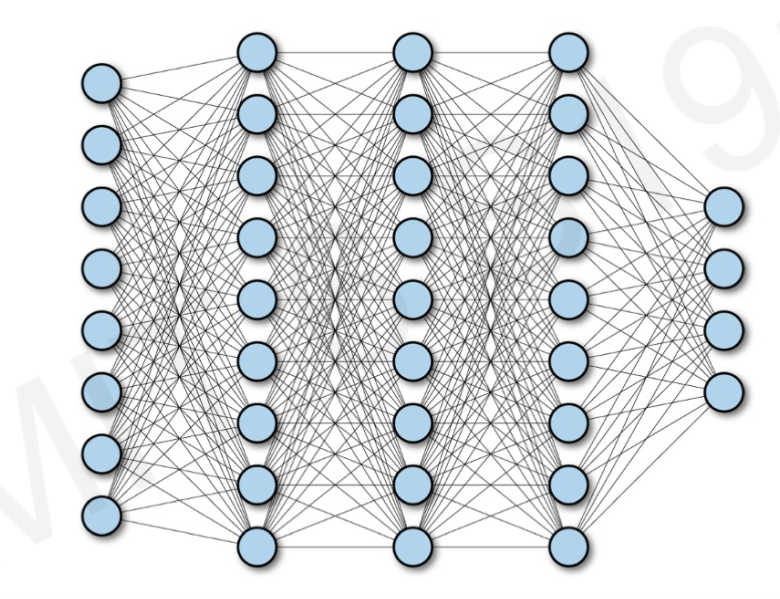
\includegraphics[scale=0.5]{img/Fully-Connected-Neural-Network.png}
            \caption{Cấu trúc FCNN}
        \end{center}
    \end{figure}

Nhược điểm của FCNN có thể thấy dễ dàng được là: 
\begin{itemize}
    \item Số lượng tham số quá nhiều, dẫn đến hao tốn nhiều tài nguyên bộ nhớ và tài nguyên tính toán của máy tính.
    \item Cấu trúc duỗi thẳng ảnh để đưa vào mạng như trên sẽ làm mất hết các đặc trưng không gian (\textit{spacial features}) của ảnh. Trong khi đó, những bài toán liên quan đến nhận diện ảnh thì các đặc trưng không gian đóng một vai trò rất quan trọng.
\end{itemize}

    \begin{figure}[H]
        \begin{center}
            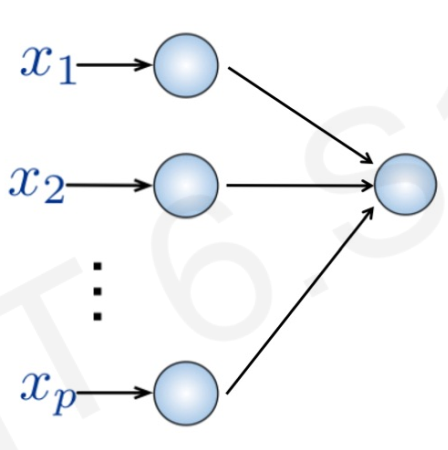
\includegraphics[scale=0.4]{img/img-to-FCNN.png}
            \caption{Input ảnh vào FCNN}
        \end{center}
    \end{figure}

Ta cần dùng một cách nào đó để có thể  đưa những đặc trưng không gian vào mô hình mạng học sâu, từ đó làm cho kết quả phân lớp ảnh của ta được cải thiện nhiều hơn.

\subsubsection{Convolution Operation}
Trong phép tích chập (\textit{Convolution Operation}), đầu vào là ảnh có kích thước $n \times n$ (F), ta sử dụng 1 bộ lọc (filter hay kernel) có kích thước $f \times f$ (h), để xuất ra ảnh có kích thước $(n - f + 1) \times (n - f + 1)$ (G).

\begin{equation}
    G = h * F
\end{equation}

\begin{equation}
    G[i, j] = \sum_{u=-f}^{f}{\sum_{v=-f}^{f}{h[u, v]F[i-u, j-v]}}
\end{equation}

    \begin{figure}[H]
        \begin{center}
            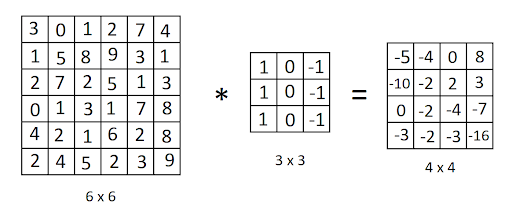
\includegraphics[scale=0.8]{img/Conv2d.png}
            \caption{Minh họa phép tích chập}
        \end{center}
    \end{figure}

Vấn đề  có thể thấy được ở phép tích chập đó là ảnh đầu ra (G) có kích thước ngày càng nhỏ. Nếu ảnh của ta đi qua nhiều lớp sẽ dẫn đến kích thước ảnh nhỏ dần làm mấy đi thông tin.

Ngoài ra, các điểm ảnh ở phần biên của ảnh đóng góp ít hơn vào các phép tích chập so với các phần tử phía bên trong của ảnh. Làm mất đi những thông tin hữu ích ở phần biên của ảnh. 

Để giải quyết vấn đề trên, người ta thêm vào xung quanh ảnh những điểm ảnh có giá trị là 0 (Có nhiều các khác nhau như giá trị mặc định hoặc điểm ảnh gần nhất), độ dày của phần điểm ảnh được thêm vào  gọi là \textit{Padding} (p)

Ngoài ra, trong một số trường hợp, ta muốn kết quả của phép tích chập cho ra ảnh có kích thước nhỏ hơn so với ảnh đầu vào. Ta định nghĩa \textit{Stride}(s) là số lượng pixel mà cửa sổ sẽ trượt qua khi thực hiện phép tích chập. Công dụng của \textit{Stride} là giảm được số lượng tham số cần phải sử dụng, nhờ đó mà tiết kiệm tài nguyên máy tính.  

Nhờ vào \textit{Padding} và \textit{Stride}, ta có thể điều khiển được kích thước của G. Ta có công thức:
\begin{equation}
    \floor*{\frac{n+2p-f}{s} + 1} \times \floor*{\frac{n+2p-f}{s} + 1}  
\end{equation}

\begin{figure}[H]
    \begin{center} 
        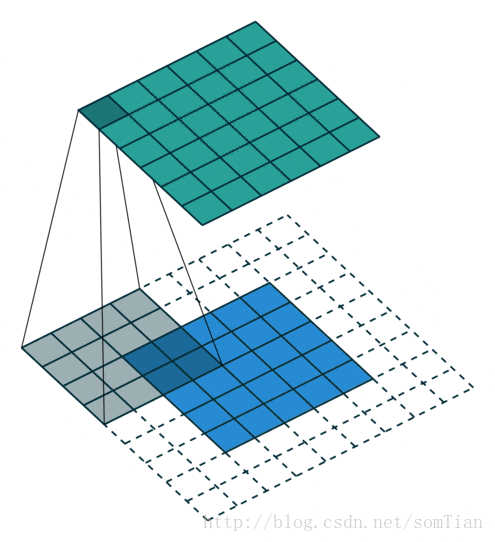
\includegraphics[scale=0.5]{img/padding-stride}
        \caption{Padding và Stride}
    \end{center}
\end{figure}

\subsubsection{Hàm Kích Họạt}
Sau khi thực hiện phép tích chập, ảnh đầu ra (G) được đưa vào 1 hàm kích hoạt (phi tuyến). Hàm này sẽ áp dụng trên mọi điểm ảnh của G và xuất ra ảnh có cùng kích thước với G. 

Có nhiều loại hàm kích hoạt khác nhau. Trong đó \textit{Rectified Linear Unit (ReLU)} được sử dung phổ  biến đối với mạng CNNs ngày nay. Các điểm ảnh  có giá trị âm khi vào \textit{ReLU} sẽ được chuyển thành 0, các điểm ảnh có giá trị lớn hơn 0 sẽ được giữ nguyên giá trị. 

\begin{figure}[H]
    \begin{center} 
        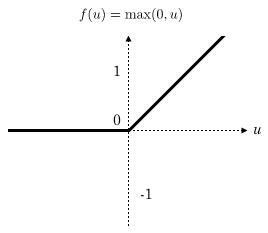
\includegraphics[scale=0.8]{img/ReLU-formula}
        \caption{Hàm kích hoạt ReLU}
    \end{center}
\end{figure}

Tác dụng của các hàm kích hoạt nói chung và của \textit{ReLU} nói riêng là giúp giới hạn giá trị của các nút mạng, tránh tình trạng bùng nổ giá trị ở các neuron. Ngoài ra, chúng còn giúp khử nhiễu, làm nổi bật lên các đặc trưng trong ảnh. Và một vấn đề  nữa là hầu như các bài toán học máy thực tế  đều là phi tuyến.

\begin{figure}[H]
    \begin{center} 
        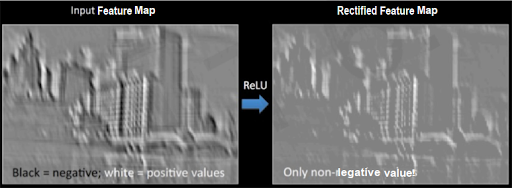
\includegraphics[scale=0.8]{img/ReLU-img}
        \caption{Thực hiện ReLU lên ảnh}
    \end{center}
\end{figure}

\subsubsection{Pooling}
Một thành phần quan trọng khác trong một mô hình CNN là các lớp \textit{Pooling}. Pooling có chức năng giảm chiều của dữ liệu. Và có thể  thực hiện phía sau một hoặc một vài lớp CONV (Convolution layers).

Trong các kĩ thuật \textit{Pooling}, kĩ thuật được sử dụng phổ biến nhất là \textit{Max Pool}. Ta thực hiện trượt một cửa sổ  kích thước $f \times f$ trên ảnh đầu vào, sau đó lấy ra điểm ảnh có giá trị lớn nhất nằm trong cửa sổ, và trượt cửa sổ qua các ô kế tiếp. 
\begin{itemize}
    \item \textit{Ví dụ:} Ảnh đầu vào có kích thước $ 4 \times 4$, và cửa số có kích thước $2 \times 2$. Kết quả sẽ là ảnh có kích thước $2 \times 2$ (Hình 17).
\end{itemize}

\begin{figure}[H]
    \begin{center}
        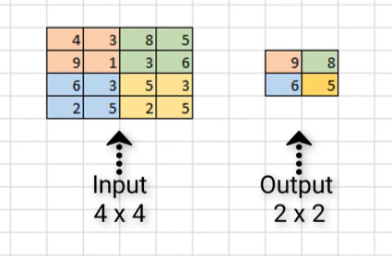
\includegraphics[scale=0.8]{img/max-pool}
        \caption{Thực hiện max pool lên ảnh có kích thước $4 \times 4$}
    \end{center}
\end{figure}

\textit{Max Pool} giúp ta giảm được kích thước ảnh, tiết kiệm tài nguyên của máy tính nhưng vẫn giữ được các đặc trưng không gian của ảnh. \textit{Max Pool} còn giúp giảm đi các vấn đề về \textit{Overfitting} do chỉ giữ lại các điểm ảnh có giá trị lớn trong từng cửa sổ giúp khử nhiễu cho ảnh. 

Ngoài \textit{Max Pool} ra, còn có rất nhiều các kĩ thuật \textit{Pooling} khác mà ta có thể tìm hiểu thêm. Ví dụ như \textit{Average Pool}, thay vì lấy giá trị lớp nhất trong cửa sổ thì \textit{Average Pool} sẽ lấy giá trị trung bình của các điểm ảnh tương ứng. \textit{Max Pool} và \textit{Average Pool} có những lợi ích khác nhau trong các bài toán cụ thể.

\subsubsection{CNNs trong bài toán phân lớp}
Bằng cách kết hợp các thành phần trên lại với nhau, ta có thể xây dựng được một mô hình CNN học các đặc trưng của ảnh một cách có cấp bậc (\textit{hierarchical}). 
\begin{itemize}
    \item \textit{Ví dụ:} Lớp CONV thứ nhất sẽ bao gồm các filter học các đặc trưng cạnh, điểm, góc,\dots của ảnh. Lớp CONV thứ hai sẽ học các đặc trưng phức tạp hơn như mắt, tai, mũi,.. Và lớp CONV thức 3 học các đặc trưng gương mặt khác nhau. (Hình 18)
\end{itemize}

\begin{figure}[H]
    \begin{center}
        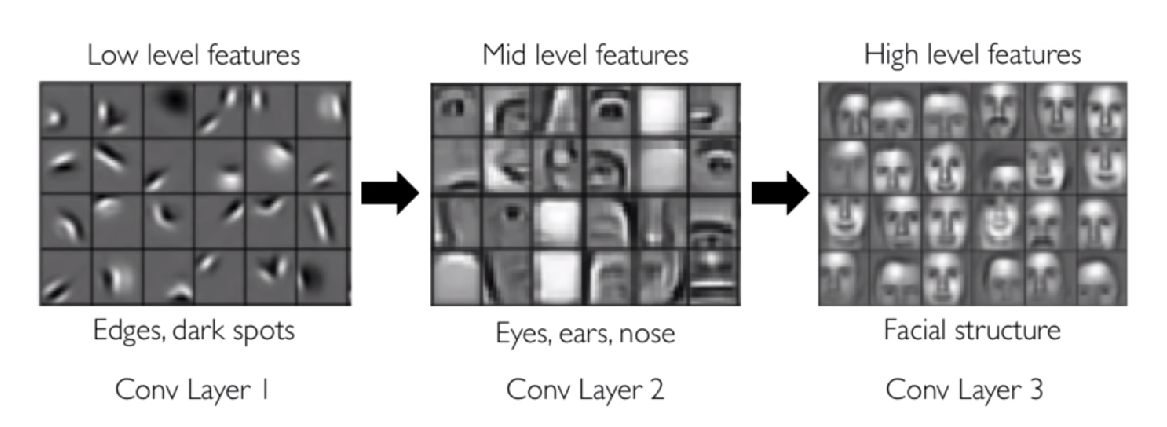
\includegraphics[scale=0.3]{img/hierarchy}
        \caption{Các đặc trưng phân cấp}
    \end{center}
\end{figure}

Một mô hình CNN trong bài toán phân lớp đươc chia ra làm 2 phần:
\begin{itemize}
    \item \textbf{Feature Learning}
    \begin{itemize}
        \item Sử dụng các lớp CONV để rút trích ra các đặc trưng quan trọng của ảnh. 
        \item Các đặc trưng được lọc qua hàm kích hoạt (ReLU) để  giới hạn miền giá trị của các pixel và giúp giải quyết vấn đề phi tuyến của ảnh (Dữ liệu phân lớp trong thực tế không tuyến tính).
        \item Giảm kích thước của ảnh nhưng vẫn giữ lại được các đặc trưng không gian của ảnh bằng các lớp POOL (Pooling layers).
            \begin{figure}[H]
                \begin{center}
                    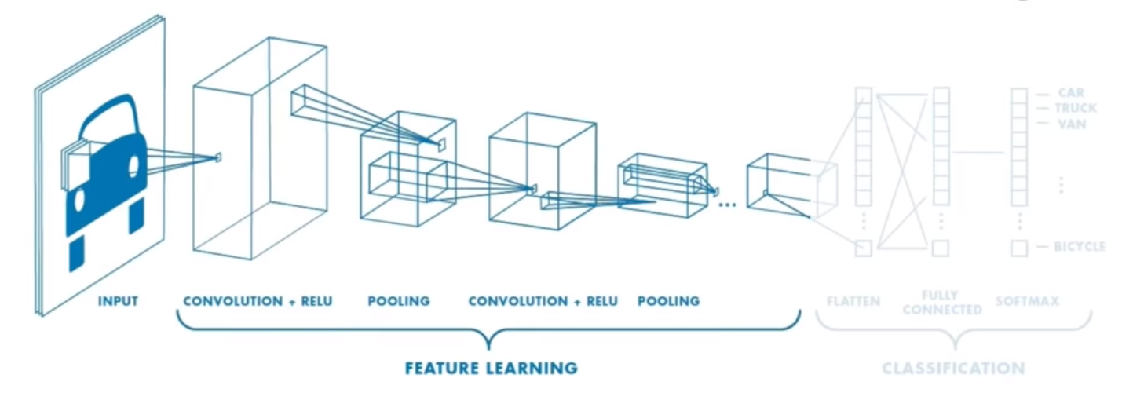
\includegraphics[scale=0.4]{img/feature-learning-part}
                    \caption{Học đặc trưng trong CNNs}
                \end{center}
            \end{figure}
    \end{itemize}
    \item \textbf{Classification}
    \begin{itemize}
        \item Sử dụng các đặc trưng được rút trích từ các lớp CONV và POOL làm đầu vào cho mô hình phân lớp. 
        \item Fully Connected Neural Network sử dụng các đặc trưng này để phân lớp cho ảnh ban đầu. 
        \item Output của phần này là xác suất ảnh ban đầu thuộc vào các lớp trong bài toán phân lớp (thường sử dụng \textit{Softmax}).
            \begin{figure}[H]
                \begin{center}
                    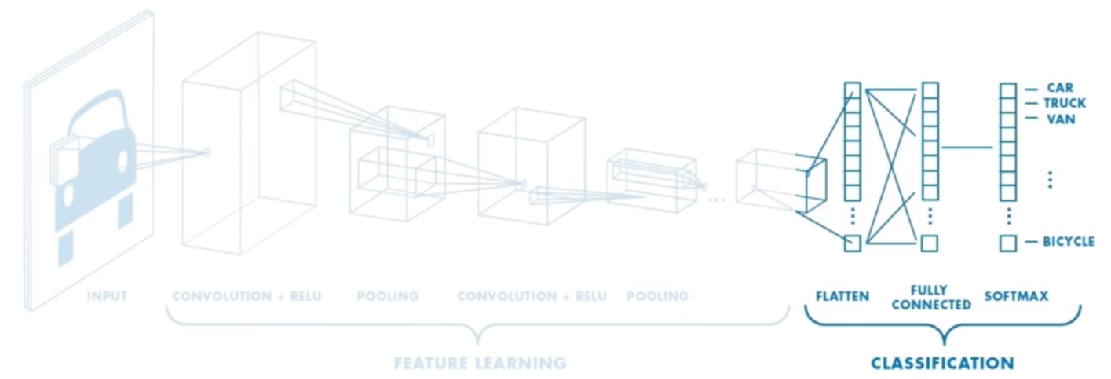
\includegraphics[scale=0.4]{img/classification-part}
                    \caption{Phân lớp trong CNN}
                \end{center}
            \end{figure}
    \end{itemize}
\end{itemize}
\subsection{Residual Network (ResNet)}
\subsubsection{Vấn đề độ sâu của các mạng học sâu}
Trên lý thuyết, nếu ta có thể tăng số lớp của mạng học sâu, ta có thể  đạt được các kết quả tốt hơn, khái quát hơn và giảm thiểu độ lỗi đáng kể. Nhưng trên thực tế , để có thể tối ưu tốt một mạng có nhiều lớp là rất khó.

    \begin{itemize}
        \item \textit{Ví dụ:} Có thể thể thấy thực nghiệm trong hình bên dưới, khi ta tăng số lớp của mạng học sâu lên, độ lỗi trên tập huấn luyện cũng tăng theo. Vấn đề mà ta gặp phải ở đây là \textit{Vanishing/Exploding Gradients}, có thể hiểu là sự thiếu hiệu quả của việc học đối với các lớp gần phía đầu của mạng trong quá trình lan truyền ngược (\textit{Backpropagation}).
            \begin{figure}[H]
                \begin{center}
                    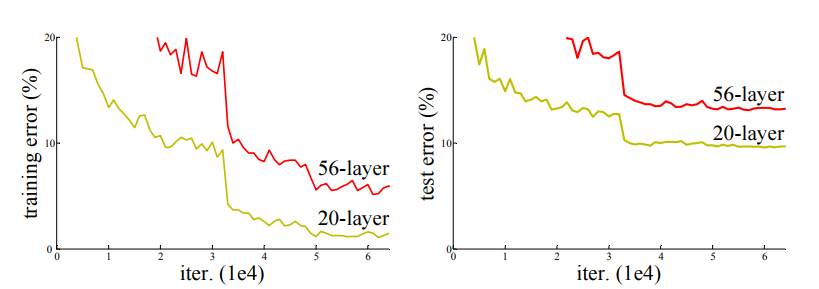
\includegraphics[scale=0.5]{img/resnet-problem}
                    \caption{Đồ thị độ lỗi trên tập huấn luyện (trái) và tập kiểm thử (phải) với mô hình CIFAR-10 (20 lớp và 56 lớp)}
                \end{center}
            \end{figure}
    \end{itemize}

\subsubsection{Skip Conection}
Khi khởi tạo một mạng học sâu, chúng ta thường khởi tạo các số có giá trị bằng 0 hoặc gần bằng 0 (Gieo ngẫu nhiên từ phân phôi chuẩn tắc) hoặc đôi khi ta còn thực hiện các kĩ thuật chuẩn hóa tham số ($L_2$ normalisation) khiến cho quá trình học ban đầu rất chậm và thậm chí còn chậm hơn nếu mạng có nhiều lớp.

Để giải quyết vấn đề này, ý tưởng của ResNet rất đơn giản, giả sử ta có một mô hình mạng học sâu gồm 2 lớp ẩn, đầu vào (x) ngoài đi theo còn luồng chính của mạng qua 2 lớp ẩn, nó sẽ được truyền theo một con đường khác và được cộng vào đầu ra của lớp thứ hai trước khi đưa vào hàm kích hoạt (\textit{ReLU}). 

Có thể thấy khi $\mathcal{F}(x)\approx 0$ thì $\mathcal{H}(x)=\mathcal{F}(x)+ x \approx x$. Nhờ vậy mà bảo toàn được các giá trị của $x$ đến các lớp sau của mạng. Một tổ hợp mạng như vậy được gọi là \textit{Residual Block}.

\begin{figure}[H]
    \begin{center}
        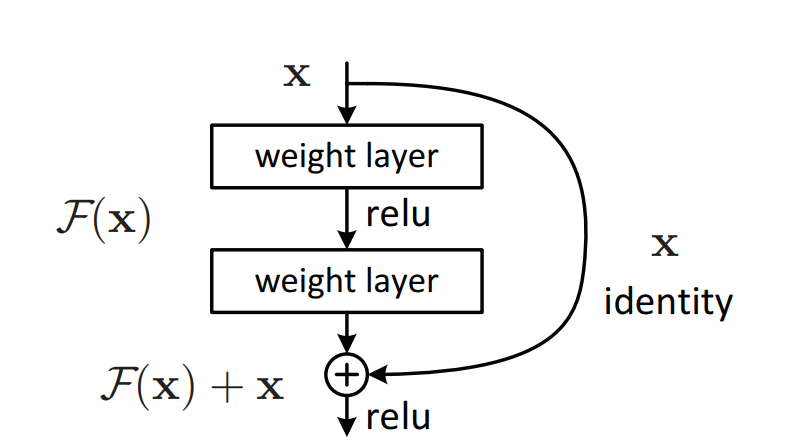
\includegraphics[scale=0.5]{img/res-block}
        \caption{Residual Block}
    \end{center}
\end{figure}

\subsubsection{Residual Network}
Bằng cách nối các \textit{Residual block} lại với nhau, ta được một mạng \textit{Residual Network}.

\begin{figure}[H]
    \begin{center}
        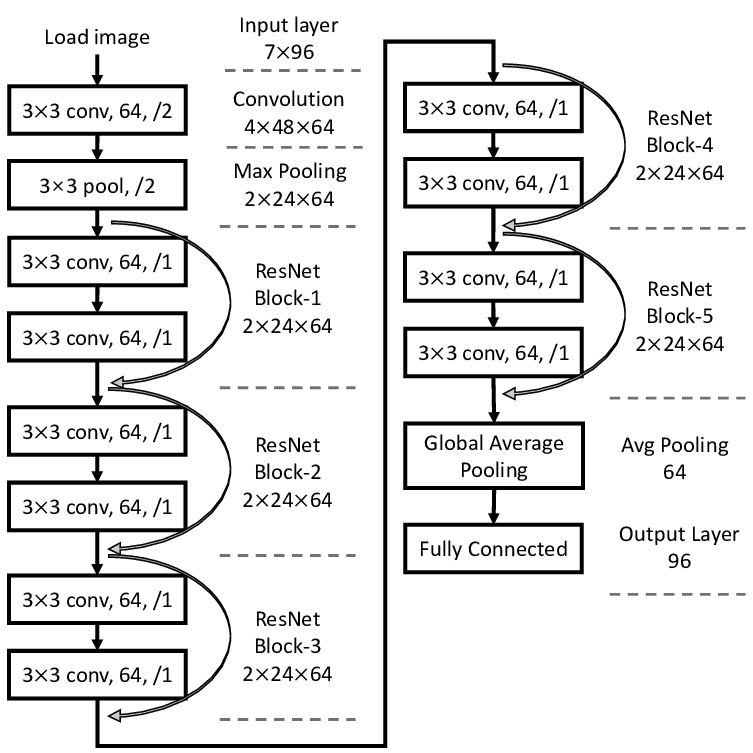
\includegraphics[scale=0.4]{img/resnet}
        \caption{Residual Network}
    \end{center}
\end{figure}

Tác giả đã thực nghiệm các so sánh trên mô hình ImageNet khi tăng số lớp từ 18 lớp đến 34 lớp. Có thể thấy khi tăng số lớp lên thì độ lỗi của mô hình không sử dụng ResNet tăng lên, trong khi đó ResNet khi tăng số lớp thì độ lỗi được giảm đi.

\begin{figure}[H]
    \begin{center}
        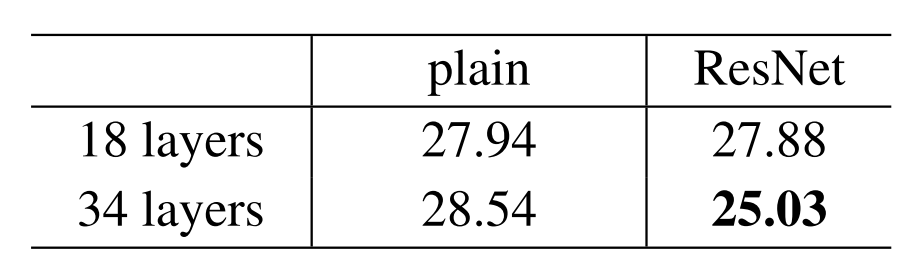
\includegraphics[scale=0.3]{img/resnet-cmp}
        \caption{Top-1 error(\%, 10-crop testing) trên tập validation}
    \end{center}
\end{figure}

\subsubsection{Bottleneck Block}
Để có thể xây dựng các mạng ResNet có độ sâu lên đến hằng trăm lớp, ta cần có 1 cấu trúc tiết kiệm tài nguyên hơn so với các \textit{Residual block}. Mỗi \textit{BottBottle block} được hình thành từ 3 lớp CONV thay vì 2 như \textit{Residual block} (Hình 25). Các lớp CONV lần lượt là $1 \times 1$, $3 \times 3$ và $1 \times 1$. Lớp CONV $1 \times 1$ đầu tiên có chức năng giảm chiều của ảnh, từ đó mà lớp CONV $3 \times 3$ có thể thực hiện phép tích chập với dữ liệu có chiều nhỏ hơn, giảm số lượng các phép tính toán. Và sau đó lớp CONV $1 \times 1$ cuối cùng khôi phục lại chiều ban đầu của của ảnh. 

\begin{figure}[H]
    \begin{center}
        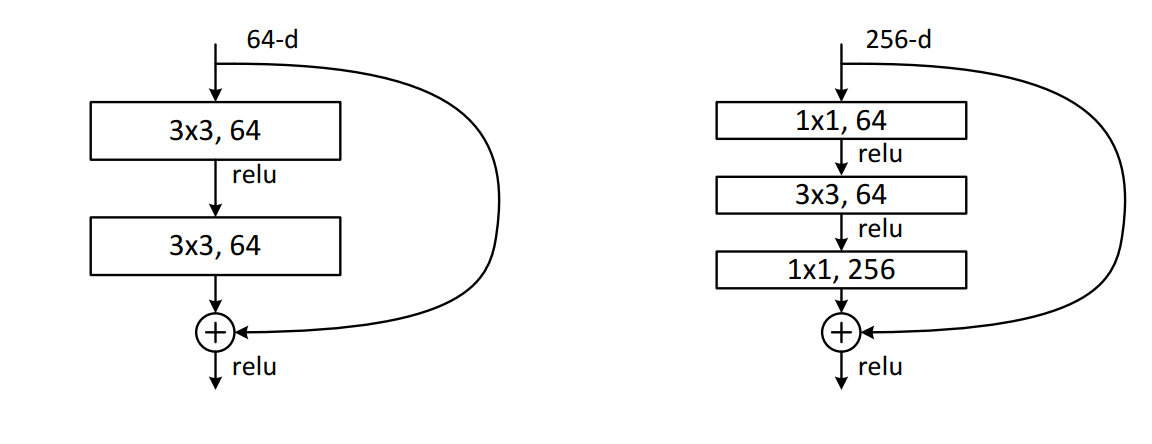
\includegraphics[scale=0.4]{img/bottleneck-block}
        \caption{Residual block ($56 \times 56$ feature maps) dùng trong ResNet-34 (trái). Bottleneck block dùng trong mạng ResNet-50/101/152.}
    \end{center}
\end{figure}
\subsubsection{Overfitting}
Tuy ResNet đã giải quyết đươc vấn đề \textit{Vanishing/Exploding Gradients}. Tuy nhiên, ResNet cũng có những hạn chế của nó. Tác giả ResNet đã thực hiện các thí nghiệm tăng số lớp của ResNet (Hình 26). Kết quả cho thấy độ lỗi trên tập test của ResNet giảm dần khi tăng số lớp lên đến 110, nhưng lại tăng lên khi tăng lên 1202 lớp. 

\begin{figure}[H]
    \begin{center}
        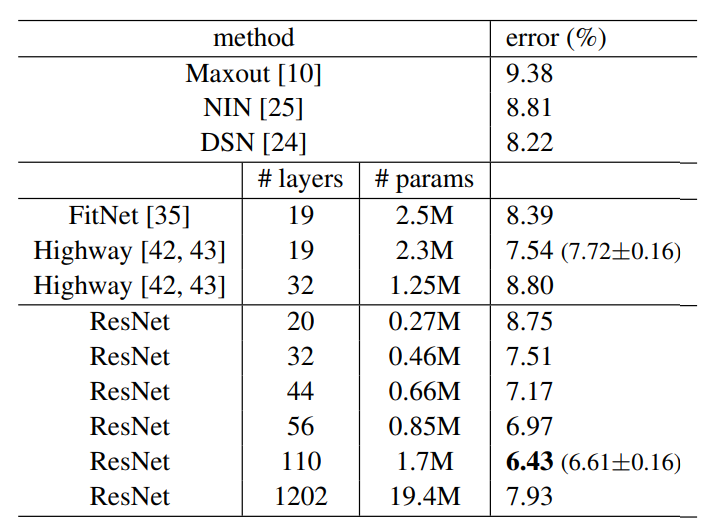
\includegraphics[scale=0.4]{img/overfitting-table}
        \caption{Độ lớp mô hình CIFAR-10 trên tập test. Các mô hình đều đươc áp dụng tăng cường dữ liệu  \textit{data augmentation}. Với ResNet-110, được chạy 5 lần và đưa ra kết quả "best(mean$\pm$std)"}
    \end{center}
\end{figure}
Có thể thấy trong hình bên dưới, độ lỗi trên tập huấn luyện của ResNet khi tăng số lớp lên ngày càng giảm, trong khi độ lỗi trên tập kiểm thử lại tăng lên. Từ đó, ta có thể khẳng định rằng, khi tăng số lớp của ResNet lên 1202 thì mô hình đã bị \textit{Overfitting}.
\begin{figure}[H]
    \begin{center}
        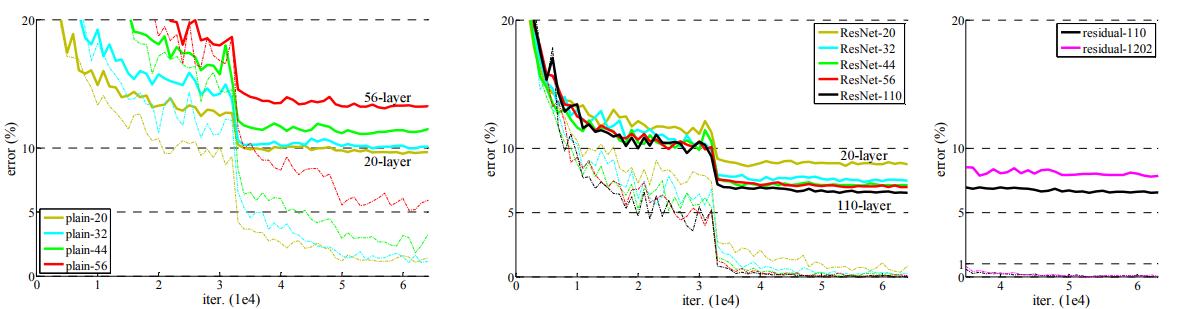
\includegraphics[scale=0.4]{img/overfitting-img}
        \caption{Huấn luyện trên CIFAR-10. Các đường nét đứt thể hiện độ lỗi trên tập huấn luyện, còn các đường in đậm thể hiện độ lỗi trên. Plain Network (trái), Residual Network(giữa), ResNet so sánh giữa 110 lớp và 1202 lớp (phải).}
    \end{center}
\end{figure}

\subsection{Additive Angular Margin Loss (ArcFace)}
\subsubsection{Hạn chế của hàm lỗi Softmax}

Softmax cho ta biết xác suất của 1 mẫu thuộc về các lớp là bao nhiêu phần trăm.
\begin{equation}
L_1=-\frac{1}{N}\sum_{i=1}^{N}{\log{\frac{e^{W_{y_i}^{T}x_i+b_{y_i}}}{\sum_{j=1}^{N}{e^{W_{j}^{T}x_i+b_{j}}}}}}
\end{equation}

\begin{figure}[H]
    \begin{center}
        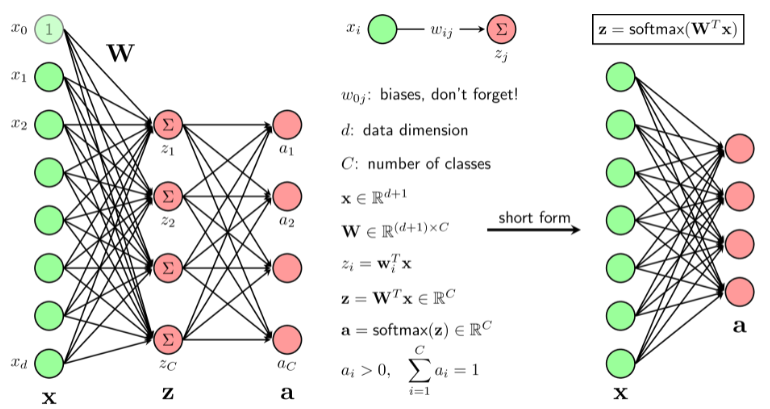
\includegraphics[scale=0.4]{img/softmax-img}
        \caption{Mô Hình Mạng Neural Softmax}
    \end{center}
\end{figure}
Nhược điểm của hàm softmax là không tối ưu tốt độ tương đồng giữa các embedding trong cùng 1 lớp và độ khác biệt giữa các lớp khác nhau. Vì thế làm giảm hiệu xuất của hệ thống phân lớp khi phương sai của lớp tăng lên (các tư thế gương mặt, biểu cảm khác nhau, sự lão hóa,\dots). Hình dưới cho ta thấy khi phải phân lớp cho các phần tử ở gần biên giữa 2 lớp \textit{class 1} và \textit{class 2} sẽ khó khăn hơn và dễ xảy ra sai sót.

\begin{figure}[H]
    \begin{center}
        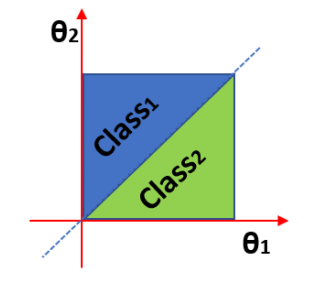
\includegraphics[scale=0.4]{img/softmax-classification}
        \caption{Hạn chế của Softmax}
    \end{center}
\end{figure}

\subsubsection{Center Loss}
Ý tưởng của \textit{Center loss} là tìm ra tâm của các lớp. Từ đó mà tối ưu khoảng cách Euclian từ các điểm dữ liệu đến tâm của lớp chứa điểm dữ liệu đó. Đồng thời cũng tối ưu khoảng cách giữa các lớp càng xa nhau.  
\begin{equation}
\mathcal{L}_C = \frac{1}{2}\sum_{i=1}^{N}\left\|x_i - c_{y_i}\right\|_2^2
\end{equation}

\begin{figure}[H]
    \begin{center}
        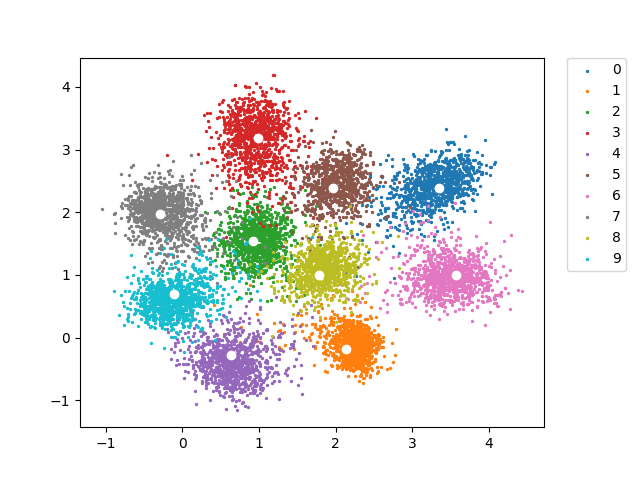
\includegraphics[scale=0.5]{img/center-loss}
        \caption{Tâm của các lớp khi dữ dụng center loss}
    \end{center}
\end{figure}

Nhược điểm của \textit{Center loss} nằm ở việc cập nhập các tâm của lớp trong quas trình huấn luyện cực kì khó khi số lượng các lớp khuôn mặt cần phải huấn luyện ngày càng nhiều lên trong thực tế.

\subsubsection{Additive Angular Margin Loss (ArcFace)}
\textit{ArcFace} hay các độ lỗi khác sử dụng góc giữa các điểm dữ liệu và các vector tham số trước đó như \textit{SphereFace} hay textit{CosFace} đã đưa ra ý tưởng sử dụng các vector tham số làm tâm của các lớp và từ đó tối ưu "khoảng cách" giữa các điểm dữ liệu đến tâm của nó. Ta có thể hình dung được rõ hơn qua công thức sau đây:
\begin{equation}
    W_{j}^{T}x_i = \|W_j\|\cdot\|x_i\|\cos{\theta_j}
\end{equation}

Với $W_j$ là vector tham số tương ứng với lớp thứ j, $x_i$ là điểm dữ liệu và $\theta_j$ là giữa giữa $W_j$ và $x_i$.  

Ta thực hiện chuẩn hóa ($L_2$ normalisation) lên các vector $W_j$ và $x_i$. Và nhân các $x_i$ với 1 lượng s. Bằng cách chuẩn hoán như trên, ta sẽ có $\|W_j\|=1$ và $\|x_i\|=s$, nhờ đó mà dự đoán khi phân lớp chỉ phụ thuộc vào $\theta_j$. Công thức (7) được đổi thành:  
\begin{equation}
L_2=-\frac{1}{N}\sum_{i=1}^{N}{\log{\frac{e^{s\cos{\theta_{y_i}}}}{e^{s\cos{\theta_{y_i}}} + \sum_{j=1,j\neq y_i}^{N}{e^{s\cos{\theta_{j}}}}}}}
\end{equation}

Từ (10), ta có thể hình dung ra các embedding sẽ tập trung xung quanh các tâm của lớp và phân bố trên 1 mặt siêu cầu (\textit{hypersphere}). Sau đó, ta cộng một siêu tham số \textit{m (Additive Angular Margin)} vào góc giữa $x_i$ và $W_j$ để có thể tối ưu tốt hơn các khoảng cách giữa các embedding. Minh hoạ bằng hình 45, ta thấy khi sử dụng hàm \textit{Softmax loss} để phân lớp, đường ranh giới giữa các lớp rất mờ, khiến cho việc phân lớp cho các điểm gần ranh giới này dễ xảy ra sai sót. Còn đối với \textit{Additive angular margin loss} bằng các sử dụng margin để ngăn cách giữa các lớp, Các điểm dữ liệu co cụm lại gần tâm của nó để  lại một khoảng cách xa giữa các lớp từ đó giúp quá trình phân lớp ít lỗi hơn.

\begin{figure}[H]
    \begin{center}
        \includegraphics[scale=0.5]{img/softmax-vs-arcface}
        \caption{So sánh giữa softmax và afcface}
    \end{center}
\end{figure}

Có thể có cai nhìn tổng quát hơn về khác biệt của các độ lỗi bằng hình bên dưới, có thể thấy các phương pháp \textit{SphereFace} và \textit{CosFace} có các đường biên quyết định (\textit{decision boundary}) có dạng phi tuyến, trong khi \textit{ArcFace} lại cho kết quả tuyến tính giúp phân lớp dễ dàng hơn.  

\begin{figure}[H]
    \begin{center}
        \includegraphics[scale=0.5]{img/loss-cmp}
        \caption{So sánh giữa giữa các độ lỗi}
    \end{center}
\end{figure}

Toàn bộ quá trình phân lớp các embedding bằng \textit{ArcFace} có thể minh họa bằng hình dưới. 

\begin{figure}[H]
    \begin{center}
        \includegraphics[scale=0.3]{img/arcface-full}
        \caption{Huấn luyện mô hình CNN sử dụng độ lỗi \textit{ArcFace}}
    \end{center}
\end{figure}

\subsection{Evaluation \& Demo}
Cuối cùng nhóm em xin được trình bày demo dữ dụng ResNet-50 + ArcFace [13], để  giải quyết bài toán Face Verification. Model được huấn luyện trên tập dữ liệu MS-CELEB-1M, và được kiếm thử trên các tập dữ liệu LFW, AgeDB-30, CFP-FP. kết quả được trình bày sau đây: 

    \begin{table}[H]
        \centering
        \begin{tabular}{|l|c|c|c|c|c|c|}
        \hline
        Backbone & Head     & Loss & Center Crop & LFW & AgDB-30 & CFP-FP\\ \hline
        ResNet-50   & ArcFace & Sofmax & False & 99.35 & 95.03 & 90.36\\ \hline
        MobileNetV2 & ArcFace & Sofmax & False & 98.67 & 90.87 & 88.51\\ \hline
        \end{tabular}
        \caption{Kết quả \textit{acuraccy} trên tập test của mô hình sử dụng ResNet-40 so sánh với MobileNetV2}
    \end{table}

\subsubsection{Demo}
Demo chúng em trình bày trong file \textit{demo.ipynb} và thực hiện các chức năng sau: 
\begin{enumerate}
    \item Xuất ra embedding sau khi chạy qua mạng. 
    \item So sánh embedding giữa cá đối tượng (ảnh được tải từ google) và cho kết quả như sau:  
    \begin{table}[H]
        \centering
        \begin{tabular}{|l|l|c|}
        \hline 
        Image 1 & Image 2 & Is same\\ \hline 
        steve.jpg & BruceLee1.jpg & False\\ \hline 
        BruceLee1.jpg & BruceLee2.jpg & True\\ \hline
        BruceLee1.jpg & TranQuocKhon.jpg & False\\ \hline 
        BruceLee2.jpg & BruceLee3.jpg & True\\ \hline
        BruceLee3.jpg & TranQuocKhon.jpg & False\\ \hline 
        \end{tabular}
        \caption{Kết quả verification trên các ảnh trong demo}
    \end{table}
\end{enumerate}

\subsection{Polynomial Neural Network($\Pi$-Net)}
\subsubsection{Xấp xỉ bằng hàm đa thức}
Nhóm tác giả của $\Pi$-Net đã chứng minh được rằng, \textit{mọi hàm số đều có thể xấp xỉ bằng một hàm đa thức}. Từ đó họ xây dựng một cấu trúc mạng không sử dụng các hàm kích hoạt phi tuyến, giúp tăng tốc độ học và độ chính xác của mạng. Một đa thức $G:\mathbb{R}^d \to \mathbb{R}^o$ bậc $N \in \mathbb{N}$ sẽ có dạng như sau:
\begin{equation}
\vb*{x} = G(\vb*{z}) = \sum_{n=1}^{N}{\left(\vb*{\mathcal{W}}^{[n]} \times_2 \vb*{b}_{[N+1-n]}\prod_{j=3}^{n+2}\times_j \vb*{z}\right)} + \vb*{\beta}
\end{equation}

Với $\vb*{z} \in \mathbb{R}^d$, $\vb*{x} \in \mathbb{R}^o$, $\{\vb*{\mathcal{W}}^{[n]} \in \mathbb{R}^{o \times w \times \Pi_m^n\times_m d}\}_{n=1}^N$, $\{\vb*{b}_{[n]} \in \mathbb{R}^{w}\}_{n=1}^{N}$ và $\vb*{\beta} \in \mathbb{R}^o$.

Nhờ vào phép phân tích CP (CP decomposition), các tensor $\vb*{\mathcal{W}}^{[n]}$ bậc cao có thể phân tích thành các tensor có bậc thấp hơn, giúp tiết kiệm được lượng tham số.

\begin{figure}[H]
    \begin{center}
        \includegraphics[scale=0.4]{img/cp-decomposition}
        \caption{CP Decomposition trên tensor 3 chiều}
    \end{center}
\end{figure}

Trong các kĩ thuật phân tích tensor mà nhóm tác giả đã đề cập thì \textit{NCP-skip (Nested coupled CP decomposition with skip)} là một kĩ thuật khá thú vị vì nó ứng dụng các nút \textit{skip connection} giống với ý tưởng của \textit{ResNet}. 

\begin{equation}
\vb*{x}_n = \left(\vb*{A}_{[n]}^{T}\vb*{z}\right) * \left(\vb*{S}_{[n]}^{T}\vb*{x}_{n-1} + \vb*{B}_{[n]}^{T}\vb*{b}_{[n]}\right) + \vb*{V}_{[n]}\vb*{x}_{n-1}
\end{equation}

Cho $n = 2,\dots,N$ với $\vb*{x}_1 = \left(\vb*{A_{[1]}^T\vb*{z}}\right) + \left(\vb*{B_{[1]}^T\vb*{b}_{[1]}}\right)$ và $\vb*{x} = \vb*{Cx}_N + \vb*{\beta}$. Các tham số $\vb*{C}\in\mathbb{R}^{o\times k}, \vb*{A_{[n]}} \in \mathbb{R}^{d \times k}, \vb*{S}_{[n]} \in \mathbb{R}^{k \times k}, \vb*{B}_{[n]} \in \mathbb{R}^{w \times k}, \vb*{b}_{[n]} \in \mathbb{R}^{w}$ và $\vb*{V}_{[n]} \in \mathbb{R}^{k \times k}$ là các tham số học.

\begin{figure}[H]
    \begin{center}
        \includegraphics[scale=0.4]{img/P-net-3rd-order}
        \caption{Mạng đa thức bậc 3}
    \end{center}
\end{figure}

\subsubsection{ProdPoly}
Thay vì sử dụng một hàm đa thức bậc cao phức tạp, ta có thể tích các đa thức có bậ thấp (2 hoặc 3) để hình thành lên các đa thức bậc cao hơn. Phép tích được thực hiện bằng cách dùng output của đa thức thứ i làm input cho đa thức thứ (i + 1).
\begin{itemize}
    \item \textit{Ví dụ:} (Hình 50) Ta sử dụng N mạng đa thức có bậc là 2 nối lại với nhau, ta sẽ được 1 mạng đa thức có bậc là $2^N$. Tổng quát hơn, nếu ta có N mạng đa thức có bậc là B , thì khi nối chúng lại với nhau ta sẽ được một mạng đa thức có bậc là $B^N$. Cấu trúc mạng như vậy được gọi là \textbf{\textit{Prodpoly}}.
\end{itemize}
\begin{figure}[H]
    \begin{center}
        \includegraphics[scale=0.4]{img/prodpoly}
        \caption{Cấu trúc mạng Prodpoly}
    \end{center}
\end{figure}

Các thí nghiệm đã được thực hiện để kiểm tra độ hiểu quả của Prodpoly so với các phương pháp ResNet trước đó. Có thể thấy Prodpoly tối ưu tốt hơn hẳn so với các mô hình chỉ sử dụng ResNet.

\begin{figure}[H]
    \begin{center}
        \includegraphics[scale=0.4]{img/resnet-vs-pnet}
        \caption{Bảng so sánh kết quả mô hình ResNet50 và Prodpoly-ResNet50}
    \end{center}
\end{figure}
\clearpage

\section{Tổng kết}
Chúng ta đã cùng nhau đi từ các phương pháp kinh điển đến hiện đại trong bài toán nhận diện gương mặt. Các kĩ thuật mới được phát triển dựa trên các mô hình mạng học sâu ngày càng thể hiện được sức mạnh của mình trong việc giải các bài toán liên quan đến nhận diện. 
Cấu trúc mạng ResNet được phát hiện vào năm 2015 và đã được phổ biến khắp các mô hình mạng học sâu. ArcFace đạt được các thứ hạng cao trong cuộc thi về nhận dạng.

\section{Tham khảo}

\begin{enumerate}
    \item \href{https://machinelearningcoban.com/2017/06/15/pca/}{Bài 27: Principal Component Analysis (machinelearningcoban)}
    \item \href{https://machinelearningcoban.com/2017/06/30/lda/}{Bài 29: Linear Discriminant Analysis(machinelearningcoban)}
    \item \href{https://machinelearningcoban.com/2017/04/09/smv/}{Bài 19: Support Vector Machine (machinelearningcoban)}
    \item \href{https://machinelearningcoban.com/2017/04/22/kernelsmv/}{Bài 21: Kernel Support Vector Machine (machinelearningcoban)}
    \item \href{http://vis-www.cs.umass.edu/lfw/}{LFW Face Dataset}
    \item \href{https://ibug.doc.ic.ac.uk/media/uploads/documents/agedb.pdf}{AgeDB Dataset}
    \item \href{http://www.cfpw.io/paper.pdf}{CFPW Dataset}
    \item \href{https://www.youtube.com/watch?v=iaSUYvmCekI}{MIT 6.S191 (2020): Convolutional Neural Networks}
    \item \href{https://www.youtube.com/playlist?list=PLkDaE6sCZn6Gl29AoE31iwdVwSG-KnDzF}{Convolutional Neural Networks (Course 4 of the Deep Learning Specialization) }
    \item \href{https://arxiv.org/pdf/1512.03385.pdf}{Residual Network}
    \item \href{https://arxiv.org/abs/1801.07698}{ArcFace: Additive Angular Margin Loss for Deep Face Recognition}
    \item \href{https://www.youtube.com/watch?v=H1qEp_czI1I&t=51s}{ArcFace explained video}
    \item \href{https://github.com/peteryuX/arcface-tf2}{ArcFace for face verification}
    \item \href{https://arxiv.org/pdf/2006.13026v2.pdf}{Polynomial Neural Network}
\end{enumerate}

\end{document}
